\subsection{Протокол <<Kerberos>>}\index{протокол!Kerberos|(}
\selectlanguage{russian}

В данном разделе будет описан протокол аутентификации сторон с единственным доверенным центром. Сетевой протокол <<Kerberos>> использует эти идеи при объединении нескольких доверенных центров в единую сеть для обеспечения надёжности и отказоустойчивости. Подробнее о сетевом протоколе <<Kerberos>> смотрите в разделе~\ref{section-kerberos}.

Как и в протоколе Нидхема~---~Шрёдера, инициирующий абонент (Алиса) общается только с выделенным доверенным центром, получая от него два пакета с зашифрованным сессионным ключом -- один для себя, а второй -- для вызываемого абонента (Боба). Однако в отличие от Нидхема~---~Шрёдера в рассматриваемом протоколе зашифрованные пакеты содержат также метку времени $T_T$ и срок действия сессионного ключа $L$ (от \langen{lifetime} -- срок жизни). Что позволяет, во-первых, защититься от рассмотренной в предыдущем разделе атаки повтором. А, во-вторых, позволяет доверенному центру в некотором смысле управлять абонентами, заставляя их получать новые сессионные ключи по истечению заранее заданного времени $L$.

\begin{figure}[!htb]
    \centering
    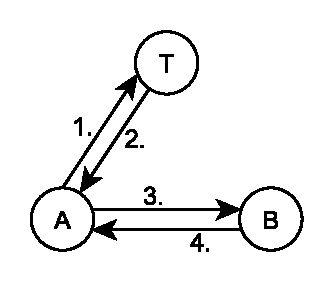
\includegraphics[width=0.5\textwidth]{pic/key_distribution-kerberos}
    \caption{Схема взаимодействия абонентов и довереного центра в протоколе <<Kerberos>>\label{fig:key_distribution-kerberos}}
\end{figure}

\begin{enumerate}
	\item $ Alice	\rightarrow \{ A, B \}									\rightarrow Trent $
	\item $ Trent	\rightarrow \{ E_A \left( T_T, L, K, B \right), E_B \left( T_T, L, K, A \right) \}	\rightarrow Alice $
	\item $ Alice	\rightarrow \{ E_B \left( T_T, L, K, A \right), E_K \left( A, T_A \right) \}		\rightarrow Bob $
	\item $ Bob	\rightarrow \{ E_K \left( T_T + 1 \right) \}						\rightarrow Alice $
\end{enumerate}

Обратите внимание, что третий шаг, за счёт использования метки времени от доверенного центра $T_T$ вместо случайной метки от Боба $R_B$ позволяет сократить протокол на один шаг по сравнению с протоколом Нидхема~---~Шрёдера. Также наличие метки времени делает ненужным и предварительную генерацию случайной метки Алисой и её передачу на первом шаге.

Интересно отметить, что пакеты $E_A \left( T_T, L, K, B \right)$ и $E_B \left( T_T, L, K, A \right)$ одинаковы по своему формату. В некотором смысле их можно назвать сертификатами сессионного ключа для Алисы и Боба. Причём все подобные пары пакетов можно сгенерировать заранее (например, в начале дня), выложить на общедоступный ресурс, предоставить в свободное использование и выключить доверенный центр (он своё дело уже сделал -- сгенерировав эти пакеты). И до момента времени $T_T + L$ этими <<сертификатами>> можно пользоваться. Но только если вы являетесь одной из допустимых пар абонентов. Конечно, эта идея непрактична -- ведь количество таких пар растёт как квадрат от числа абонентов. Однако интересен тот факт, что подобные пакеты можно сгенерировать заранее. Эта идея нам пригодится при рассмотрении инфраструктуры открытых ключей (\langen{public key infrastructure, PKI}).

\index{протокол!Kerberos|)}